%\part{Rapport~1}

\section{Bilan de masse (rapport 1)}

Nous faisons l'hypothèse que la réaction est parfaite, 
c'est-à-dire que tous les réactifs sont consommés 
et que l'on obtient uniquement le produit.

Il faut déterminer la quantité de dihydrogène (\ce{H2}) et d'azote (\ce{N2}) 
nécéssaire pour produire $1000 \si{\tonne}$ d'ammoniac (\ce{NH3}).

\begin{equation}
	\ce{\frac{3}{2} \, H2 + \frac{1}{2} \, N2 -> NH3} 
	\label{eq:ammoniac}
\end{equation}

La masse molaire de l'ammoniac vaut $17 \si{\gram\per\mole}$,
il faut donc en produire $5.88\e{7} \si{\mole}.$

On obtient les nombres de moles de réactifs à partir de la réaction pondérée. 

\begin{align*}
	m_{\ce{H2}}  = \frac{3}{2} \, n_{\ce{NH3}} \cdot M_{m, \ce{H2}} 
	= 1.765\e{8} \si{\gram} \\
	m_{\ce{N2}} = \frac{1}{2} \, n_{\ce{NH3}} \cdot M_{m, \ce{N2}} 
	= 8.235\e{8} \si{\gram}
\end{align*}

Les masses de \ce{H2} et de \ce{N2} valent donc 
respectivement $176.5 \si{\tonne}$ et $823.5 \si{\tonne}$.
Le bilan de masse est correct : si on fait la somme des masses des réactifs,
on retrouve la même masse produite.

\section{Débit d'eau nécessaire}

Afin de maintenir les réacteurs à température constante, 
on refroidit ceux-ci avec de l'eau.
Il faut tout d'abord calculer la chaleur dégagée par jour par les réacteurs,
pour ensuite déterminer la quantité d'eau nécessaire pour absorber cette chaleur,
sachant que l'eau entre à $25 \si{\degreeCelsius}$ et 
est évacuée à $90 \si{\degreeCelsius}$.
Les calculs suivants sont présentés pour une quantité d'ammoniac de $1000\si{\tonne}$ par jour, 
la fonction \texttt{refroidissement} permet d'avoir le débit nécessaire (en litres par seconde) 
en fonction de la quantité de \ce{NH3} désirée.

\paragraph{In}

La chaleur dégagée par la réaction \ref{eq:ammoniac} correspond à la 
différence entre l'enthalpie de formation des produits et celle des réactifs. 

\begin{equation}
	\Delta H_{réaction} = \Delta H_{f, \ce{NH3}} 
	- \frac{1}{2} \Delta H_{f, \ce{N2}}
	- \frac{3}{2} \Delta H_{f, \ce{H2}}
	\label{eq:enthalpie_reaction}
\end{equation}

La réaction se passe à $500 \si{\degreeCelsius}$, 
on détermine donc les $\Delta H_{f}$ des différents 
composés à partir des valeurs des enthalpies standard
de formation \cite{atkins} (à $25 \si{\degreeCelsius}$)
et des capacités calorifiques molaires ($C_p$), gr\^ace 
à l'équation suivante:

\begin{equation*}
	\Delta H_{f, T2} = \Delta H_{f, T1} 
	+ \int_{T1}^{T2} C_p \, \dif{T}
\end{equation*}

Étant donné que nous travaillons avec des quantités importantes de matière,
nous ne pouvons pas considérer que $C_p$ est constant.
On sait que $C_p$ varie en fonction de la température 
selon une fonction $a + b T + c T^2$, 
où $a$, $b$ et $c$ sont des constantes \cite{capcaloUPMC}. 

Nous pouvons à présent calculer les enthalpies 
de formation à $500 \si{\degreeCelsius}$

\begin{equation}
	\Delta H_f = \Delta H_{f}^{\si{\degree}} + 
	\int_{298}^{773} (a + b T + c T^2) \, \dif{T}
	\label{eq:enthalpie_500C}
\end{equation}

À partir de l'équation \ref{eq:enthalpie_500C}, 
on obtient les valeurs suivantes

\begin{align*}
	\Delta H_{\ce{H2}} &= 14 \, \si{\kilo\joule\per\mole} \\
	\Delta H_{\ce{N2}} &= 14.19 \, \si{\kilo\joule\per\mole} \\
	\Delta H_{\ce{NH3}} &= -26.21 \, \si{\kilo\joule\per\mole} 
\end{align*}

Pour finir, on trouve l'enthalpie de réaction par l'équation \ref{eq:enthalpie_reaction}

\[
	\Delta H_{reaction} = -54.31 \, \si{\kilo\joule\per\mole}
\]

\paragraph{Out}

Le raisonnement pour la chaleur absorbée est similaire 
au précédent, sauf que cette fois ci, 
on considère que la capacité calorifique est constante.
Cette hypothèse peut être raisonnablement envisagée 
étant donné que \cite{janaf}
$C_{p, 298 \si{\kelvin}} \approx 75.35 \, \si{\joule\per\kelvin\per\mole}$ 
et $C_{p, 368 \si{\kelvin}} \approx 75.78 \, \si{\joule\per\kelvin\per\mole}$.
La différence étant très petite, 
nous prendrons la moyenne de ces deux valeurs. 

La chaleur absorbée par une mole d'eau vaut exactement

\begin{equation}
	\Delta H = \int_{298}^{363} C_{p, \ce{H2O}} \, \dif{T}
	= 75.565 \cdot 65 = 4911.73 \, \si{\joule\per\mole}
\end{equation}

\paragraph{Débit}

Il s'agit maintenant de déterminer la quantité d'eau nécessaire par jour.
Il faut que

\[
	\frac{\Delta H_{in}}{\mathrm{jour}} 
	= - \frac{\Delta H_{out}}{\mathrm{jour}}
\]

En sachant qu'on produit $1000 \si{\tonne}$ de \ce{NH3} par jour
(cela équivaut à $5.88\e{7} \, \si{\mole}$),
et à partir des données trouvées ci-dessus, 
on trouve que

\begin{align*}
	n_{\ce{H2O}} &= \frac{n_{\ce{NH3}} \, \Delta H_{in}}{\Delta H_{out}} \\
	&= 6.5\e{8} \si{\mole} 
\end{align*}

Il faut donc $11703 \si{\tonne}$ d'eau par jour, 
ou encore 136 litres par seconde.


%\part{Rapport~2}

\section{Introduction}

Ce second rapport est une extension et une amélioration du rapport rendu 
en S2 et a pour but d'étudier plus en détail la production d'ammoniac. 
Il comprend un flow sheet qui permet de voir les flux de matières en 
les différentes étapes de la synthèse par le procédé Haber-Bosh. 
Il comprend aussi un calcul détaillé des aspects énergétiques dans le réformateur primaire.
S’y trouve ensuite une explication du fonctionnement de l’outil de calcul
réalisé sur \textsc{matlab} (ainsi que l'outis de calcul en annexe).
Celui-ci permet le calcul des flux entrants et sortants en fonction 
de la quantité d'ammoniac voulue dans la journée ainsi que de la 
température dans le réformateur primaire. Il calcule également les aspects énergétiques 
lors des différentes étapes. 
Et enfin ce rapport se termine par une analyse de l'effet du changement 
des variables que sont la température et la quantité d'ammoniac produite 
sur le bilan de matière.

\section{Bilan de matière}
\label{sec:bilan_matiere}

Une partie de la t\^ache 1 consiste à réaliser un outil de gestion
pour pouvoir déterminer les quantités de matières premières nécessaires,
lorsque 2 paramètres varient. 
Les paramètres sont la température à la sortie de réacteur primaire ainsi
que la quantité d'ammoniac produite par jour. 
On les notera respectivement $T$ et $m_{\ce{NH3}}$.

À travers cette section, nous décrirons différentes réactions et nous 
supposons que le lecteur sait quelle réaction a lieu à quel moment ainsi 
que l'ordre des réactions durant tout le processus.
Un flow-sheet simplifié de l'ensemble du processus détaillant chacune
des réactions se trouve à la section \ref{sec:flowsheet}.

\subsection{Quantité d'air}

Nous connaissons la masse d'ammoniac à produire par jour, 
et par conséquent son nombre de moles ($n_{\ce{NH3}} = m_{\ce{NH3}}/M_{\ce{NH3}}$).
Les nombres de moles seront généralement écrits en fonction de $m_{\ce{NH3}}$ 
de façon à montrer la relation par rapport au paramètre qui varie.

À partir de la réaction suivante,

\begin{equation*}
	\ce{\frac{3}{2} \, H2 + \frac{1}{2} \, N2 -> NH3} 
\end{equation*}

on détermine les quantités de \ce{H2} et de \ce{N2} nécessaires.

\begin{align}
	n_{\ce{H2}} = \frac{3}{34} \, m_{\ce{NH3}} 
	\label{eq:moles_H2} \\
	n_{\ce{N2}} = \frac{1}{34} \, m_{\ce{NH3}} \nonumber
\end{align}

Or la seule source d'azote est lorsque l'air entre dans le réacteur secondaire.
En connaissant les proportions de l'azote, de l'oxygène et de l'argon dans 
l'air, on peut facilement obtenir les quantités de \ce{O2} et de \ce{Ar}.

\begin{align*}
	n_{\text{air}} = \frac{1}{0.78} \, n_{\ce{N2}} = \frac{25}{663} \, m_{\ce{NH3}} \\
	n_{\ce{O2}} = 0.21 \, n_{\text{air}} = \frac{7}{884} \, m_{\ce{NH3}} \\
	n_{\ce{Ar}} = 0.01 \, n_{\text{air}} = \frac{1}{2652} \, m_{\ce{NH3}} 
\end{align*}

\subsection{Quantité de méthane et d'eau}

Il nous reste maintenant à déterminer les quantités de \ce{CH4} et de \ce{H2O}.
On voit que la seule réaction nécessitant de l'oxygène est celle du 
réformage secondaire. Ceci nous permet de conna\^itre toutes les quantités 
associées à cette réaction. 
Afin de ne pas oublier à quelle réaction est associée chaque quantité, 
on notera \textit{rp} (resp. \textit{rs}) pour réformage primaire (resp. secondaire)
et \textit{wgs} pour Water-Gas-Shift.

\begin{equation*}
	\ce{2CH4 + O2 -> 2CO + 4H2}
\end{equation*}

Dès lors, 

\begin{align}
	n_{\ce{CO}, rs} = n_{\ce{CH4}, rs} 
	= 2 \, n_{\ce{O2}} = \frac{7}{442} \, m_{\ce{NH3}} 
	\label{eq:moles1_ref_sec} \\
	n_{\ce{H2}, rs} = 4 \, n_{\ce{O2}} = \frac{7}{221} \, m_{\ce{NH3}}
	\label{eq:moles2_ref_sec}
\end{align}

Interessons nous maintenant au réformage primaire.
\begin{align*}
	&\ce{CH4 + H2O <-> CO + 3H2} \\
	&\ce{CO + H2O <-> CO2 + H2}
\end{align*}

Comme les deux réactions sont à l'équilibre,
il va falloir déterminer leurs constantes d'équilibres sans
oublier qu'elles s'influencent mutuellement.
C'est ici qu'intervient le paramètre $T$. On va donc commencer
par calculer les $\Delta_r G^{\circ}$ afin de conna\^itre les constantes
d'équilibres $K(T)$, pour finalement déterminer les quantités des différents composés
à l'équilibre.

\paragraph{Calcul des constantes d'équilibres $K(T)$}

On a déjà vu précedement que les valeurs des capacités calorifiques
à pression constante varient avec la température. Afin d'avoir un outil de gestion
le plus précis possible, nous allons utiliser les équations de Shomate pour calculer 
les enthalpies et entropies standards. 
Lors du précédent rapport, nous avions décris que $C_{p,m}^{\circ} = A + B \, T + C \, T^2$,
on ajoute un degré de précision en posant

\begin{equation}
	C_{p,m}^{\circ} = A + B \, t + C \, t^2 + D \, t^3 + \frac{E}{t^2}
	\quad \text{avec} \quad t = \frac{T[K]}{1000}
	\label{eq:shomate}
\end{equation}

les valeurs des différents coefficients\footnote{Il faut ajouter deux autres 
coefficients F et G à cause des constantes d'intégrations pour les
enthalpies et entropies.} 
se trouvent \cite{shomate} dans la fonction \texttt{getCoefficients}.
On en déduit donc les valeurs des enthalpies et entropies
à partir de l'équation \ref{eq:shomate} dans la fonction \texttt{getDeltaH\_and\_S}  

\begin{align*}
	\Delta_f H_{T2}^{\circ} &= \Delta_f H_{T1}^{\circ} 
	+ \int_{T1}^{T2} C_{p,m} \, \dif{T} \\ 
				 &= \Delta_f H_{T1}^{\circ} 
	+ A \, t + B \, \frac{t^2}{2}  + C \,  \frac{t^3}{3} 
	+ D \, \frac{t^4}{4} - \frac{E}{t} + K_{1} \\		 
	S_{T2}^{\circ}  &= S_{T1}^{\circ} + \int_{T1}^{T2} 
	\frac{C_{p,m}}{T} \, \dif{T} \\
			&= S_{T1}^{\circ} + A \, \ln{t} 
	+ B \, t + C \, \frac{t^2}{2} 
	+ D \, \frac{t^3}{3} - \frac{E}{2 t^{2}} + K_{2} 
\end{align*}

Afin de ne pas trop alourdir ce document, les détails des calculs sont ignorés. 

On détermine ensuite l'enthalpie libre de Gibbs via la relation 

\begin{equation*}
	\Delta_r G^{\circ} = \Delta_r H^{\circ} 
	- T \, \Delta_r S^{\circ}
\end{equation*}

et finalement la constante d'équilibre 

\[ 
K(T) = \exp{\left(\frac{- \Delta_r G}{R \, T}\right)} 
\]

Les constantes d'équilibre des deux réactions du réformage primaire 
sont calculées dans la fonction \texttt{getEqConstantsRef}.

\paragraph{Calcul des pressions partielles à l'équilibre}

Les tableaux \ref{tab:reaction1_primaire} et \ref{tab:reaction2_primaire} nous 
permettent de conna\^itre les quantités des réactifs et des produits à l'équilibre. 

\begin{table}
	\centering
	\begin{tabular}{l|c|c|c|c|c}
		 & $\ce{CH4}$ & $\ce{H2O}$ & $\ce{CO}$ & $\ce{3H2}$ & $n_{gaz}$ \\
		\hline
		$p_{i}$ & $n_{\ce{CH4}}$ & $n_{\ce{H2O}}$ & $0$ & $0$ &
		$n_{\ce{CH4}} + n_{\ce{H2O}}$ \\
		$p_{eq}$ & $n_{\ce{CH4}} - \xi_1$ & $n_{\ce{H2O}} - \xi_1$ & 
		$\xi_1$ & $3 \, \xi_1$ & $n_{\ce{CH4}} + n_{\ce{H2O}} + 2 \, \xi_1 $\\
	\end{tabular}
	\caption{Première réaction du réformage primaire à l'équilibre}
	\label{tab:reaction1_primaire}
\end{table}

\begin{table}
	\centering
	\begin{tabular}{l|c|c|c|c|c}
		 & $\ce{CO}$ & $\ce{H2O}$ & $\ce{CO2}$ & $\ce{H2}$ & $n_{gaz}$ \\
		\hline
		$p_{i}$ & $\xi_1$ & $n_{\ce{H2O}} - \xi_1$ & $0$ & $3 \, \xi_1$ &
		$n_{\ce{H2O}} + 3 \, \xi_1$ \\
		$p_{eq}$ & $\xi_1 - \xi_2$ & $n_{\ce{H2O}} - \xi_1 - \xi_2$ & 
		$\xi_2$ & $3 \, \xi_1 + \xi_2$ & $n_{\ce{H2O}} + 3 \, \xi_1 $\\
	\end{tabular}
	\caption{Deuxième réaction du réformage primaire à l'équilibre}
	\label{tab:reaction2_primaire}
\end{table}

Il s'agit maintenant de résoudre 4 équations afin de déterminer nos inconnues que 
sont $\xi_1$, $\xi_2$, $n_{\ce{CH4}}$ et $n_{\ce{H2O}}$. 
On a tout d'abord les deux liées aux activités et constantes $K$, que nous déduisons
à partir des informations des réactions à l'équilibre.

\begin{align}
	K_1 &= \frac{p_{tot}^2 \, (\xi_1 - \xi_2) \, (3 \xi_1 + \xi_2)^3}
	{p_{0}^2 \, (n_{\ce{CH4}} + n_{\ce{H2O}} + 2 \xi_2)^2 \, (n_{\ce{CH4}} - 
	\xi_1) \, (n_{\ce{H2O}} - \xi_1 - \xi_2 )} 
	\label{eq:systeme1} \\
	K_2 &= \frac{\xi_2 \, (3 \xi_1 + \xi_2)}
	{(\xi_1 - \xi_2) \, (n_{\ce{H2O}} - \xi_1 - \xi_2)}
	\label{eq:systeme2}
\end{align}

Les deux suivantes s'appuyent sur le fait que si une mole d'un composé $X$ est
produite à une réaction $\alpha$, une mole de ce même composé sera disponible 
dans la réaction suivante.

On a pu voir dans le tableau \ref{tab:reaction1_primaire} qu'il reste après 
équilibre exactement $n_{\ce{CH4}} - \xi_1$ moles de \ce{CH4}, qui seront 
entièrement consommées pendant le réformage secondaire. 
Par l'équation \ref{eq:moles1_ref_sec}, on a que 

\begin{equation}
	n_{\ce{CH4}} - \xi_1 = \frac{7}{442} \, m_{\ce{NH3}}
	\label{eq:systeme3}
\end{equation}

Pour finir, on remarque que 

\begin{equation*}
	n_{\ce{H2}} = n_{\ce{H2}, rp} + n_{\ce{H2}, rs} + n_{\ce{H2}, wgs}
\end{equation*}

on vient de voir (tableau \ref{tab:reaction2_primaire})
que $n_{\ce{H2}, rp} = 3 \, \xi_1 + \xi_2$, nous connaissons égalemment
$n_{\ce{H2}}$ (équation \ref{eq:moles_H2})
et $n_{\ce{H2}, rs}$ (équation \ref{eq:moles2_ref_sec}), on a ensuite 

\begin{align*}
	n_{\ce{H2}, wgs} = n_{\ce{CO}, \text{total}} 
	&= n_{\ce{CO}, rp} + n_{\ce{CO}, rs} \quad &\text{(voir flow-sheet)} \\
	&= \xi_1 - \xi_2 + \frac{7}{442} \, m_{\ce{NH3}} 
	\quad &\text{(voir tableau \ref{tab:reaction2_primaire} et eq \ref{eq:moles1_ref_sec})}
\end{align*}

Ce qui nous donne 

\begin{equation}
	4 \, \xi_1 = \frac{9}{221} \, m_\ce{NH3}
	\label{eq:systeme4}
\end{equation}

Nous résolvons le système de 4 équations 
(\ref{eq:systeme1}, \ref{eq:systeme2}, \ref{eq:systeme3}, \ref{eq:systeme4})
dans \texttt{solveG}.

\section{Fonctionnement de l'outil de calcul}

L'outil de calcul a été réalisé en matlab et prends en considération 
deux variables : la température du réacteur primaire (en K) et la quantité 
d'ammoniac (en tonnes) que l'on souhaite produire en 24h. 

Nous commençons tout d'abord par calculer les enthalpies (incl. Gibbs) 
et entropies des réactions du réacteur primaire (vaporeformage).
Nous calculons ensuite les constantes d'équilibres pour les deux réactions. 
Avec les hypothèses posées sur les réactions (toutes sont complètes 
exceptées celles s'effectuant dans le réacteur primaire),
et avec la masse désirée de \ce{NH3}, nous calculons les masses 
nécessaires de \ce{H2}, \ce{N2}. Puisque l'azote est fourni
par l'air, nous déterminons la masse de \ce{O2} fournie (ainsi que la masse de \ce{Ar}, 
mais l'argon est un gaz noble et n'intervient pas dans la réaction). 

Avec les hypothèses et la masse de \ce{O2}, nous déterminons la quantité de \ce{CH4} 
utilisé dans le réacteur secondaire et donc la production de \ce{H2} dans ce réacteur. 
Nous savons désormais déterminer la quantité de \ce{H2} à produire dans 
le réacteur primaire, et grâce à la constante d'équilibre déterminée plus tôt, 
nous pouvons déterminer la quantité de \ce{CH4} nécessaire pour les deux réactions.
L'outil nous permet également de calculer la quantité minimum de \ce{H2O} à fournir
pour que toutes les équations se passent comme prévu. 

Il est à noter que l'outil nous fourni des valeurs en tonnes par jour.

\section{Tubes}

Nous recherchons le nombre de tubes nécessaire à l'acheminement du 
méthane et de l'eau dans le reformateur primaire.

Soit $x$ le nombre de tubes, nous avons l'équation suivante :
\[
	\dot{V} = A \, \dot{c} \, x
\]

Avec $\dot{V}$ le débit, $A$ la section d'un tuyau 
et $\dot{c}$ la vitesse superficielle à l'entrée du réacteur.
Le volume peut être calculé grâce à la loi des gaz parfaits,
on considère donc que \ce{H2O} se comporte comme un gaz parfait,
pour plus de précision on pourra éventuellement utiliser l'équation
d'état de van der Waals.
\[
	V = \frac{n R T}{p}
\]

Si l'on considère notre calcul en un temps d'une seconde, 
la simplification des deux formules ci-dessus nous amène à
\[
	x = \frac{n R T}{A \dot{c} \, p}
\]

Or nous savons que la vitesse superficielle à l'entrée des tubes 
vaut $2 \si{\meter\per\second}$,
que leurs diamètre est de $1 \si{\centi\meter}$ 
(la section d'un tube est $A = \pi r^2$),
et qu'il y a une pression de $31 \si{\bar}$ à l'entrée.
Les seules inconnues sont donc la température et les nombres de moles
de produit entrant, c'est-à-dire de \ce{CH4} et de \ce{H2O},
que nous avons déterminé dans la section \ref{sec:bilan_matiere}.

Prenons l'exemple, pour une quantité d'ammoniac de $1500 \si{\tonne}$ 
(toujours avec une température du réformeur primaire de $1000\si{\kelvin}$
et une pression à l'entrée de $28\si{\bar}$).

\begin{align*}
	n_{\ce{CH4}} = 451.70 \si{\mole\per\second} \\
	n_{\ce{H2O}} = 936.95 \si{\mole\per\second}
\end{align*}

Grâce aux autres valeurs données dans l'énoncé 
nous pouvons calculer le nombre de tubes nécessaire 

\[
 x = \frac{(n_{\ce{CH4}}+n_{\ce{H2O}}) \cdot 8,314 \cdot 1000}
	{\pi (0,05^2) \cdot 2 \cdot (31.10^5)} = 237.1
\]

Il faut donc $238$ tuyaux pour assurer l'approvionnnement 
des composés dans le reformateur primaire.

La fonction \texttt{getTubesNumber} donne le
nombre de tubes requis en fonction des paramètres de départ (la masse d'ammoniac 
à produire, la température du réformeur primaire ainsi que la pression de celui-ci).

\section{Bilan énergétique de la partie réformeur primaire-four}

La première réaction - le craquage du méthane - qui se produit dans le réformeur primaire,
est une réaction endothermique. Nous devons donc lui fournir de l'énergie sous 
forme de chaleur, ce r\^ole va être rempli par le four. 
La réaction de combustion qui a lieu dans le four est la suivante

\[
	\ce{CH4 + 2O2 -> CO2 + 2H2O}
\]

Afin de connaître les quantités de méthane et d'oxygène qu'il faut
introduire dans le four, nous devons étudier les bilans énergétiques
des réactions ayant lieu dans ce réformateur. Les calculs exposés dans cette section 
sont fait pour une température dans le réformateur de $1080 \si{\kelvin}$
et pour une production journalière d'ammoniac de $1500 \si{\tonne}$. 
Bien sur ces résultats sont facilement transposables
à d'autres données à l'aide de notre outil de gestion.

Il faut tout d'abord calculer la chaleur nécessaire dans le réformeur primaire.
La différence d'enthalpie de réaction du craquage du méthane vaut $+225.7 \si{\kilo\joule}$
à $1000 \si{\kelvin}$, et celle de la deuxième réaction
vaut $-34.8 \si{\kilo\joule}$ à la même température.
La première est fortement endothermique tandis que la deuxième est exothermique.
Il faut fournir une quantité de chaleur $Q$ pour que la réaction endothermique
puisse avoir lieu, tout en tenant compte que le rendement énergétique de 
la réaction de combustion du four vaut $\eta = 0.75$.
Le nombre de moles qui vont réagir dans les réactions du réformeur primaire 
sont $\xi_1$ et $\xi_2$ (tableaux \ref{tab:reaction1_primaire} 
et \ref{tab:reaction2_primaire}).

On a donc que 
\[
	Q = n_{\ce{CH4},\text{four}} \cdot \Delta_r H_{\text{four}} \cdot \eta
\]

et 
\[
	-Q = \xi_1 \cdot \Delta_r H_{rp,1} + \xi_2 \cdot \Delta_r H_{rp,2}
\]

On obtient une équation à résoudre pour obtenir $n_{\ce{CH4},\text{four}}$, et on a ensuite
les quantités à introduire (\ce{O2}) et celles rejetées (\ce{CO2} et \ce{H2O})
\begin{align*}
	n_{\ce{O2},\text{four}} &= 2 \cdot n_{\ce{CH4},\text{four}} \\
	n_{\ce{CO2},\text{four}} &= n_{\ce{CH4},\text{four}} \\
	n_{\ce{H2O},\text{four}} &= 2 \cdot n_{\ce{CH4},\text{four}}
\end{align*}

On en déduit ensuite facilement la quantité d'air à introduire.
Ce bilan énergétique est modélisé dans \texttt{getHovenMasses}.

\section{Analyse Paramétrique}

On observe sur la figure~\ref{fig:analyseParam} qu'il y a seulement l'eau 
qui varie avec la température.
Les autres composés ne varient donc qu'avec la quantité de \ce{NH3} à produire.

\begin{figure}[h!]
	\begin{center}
		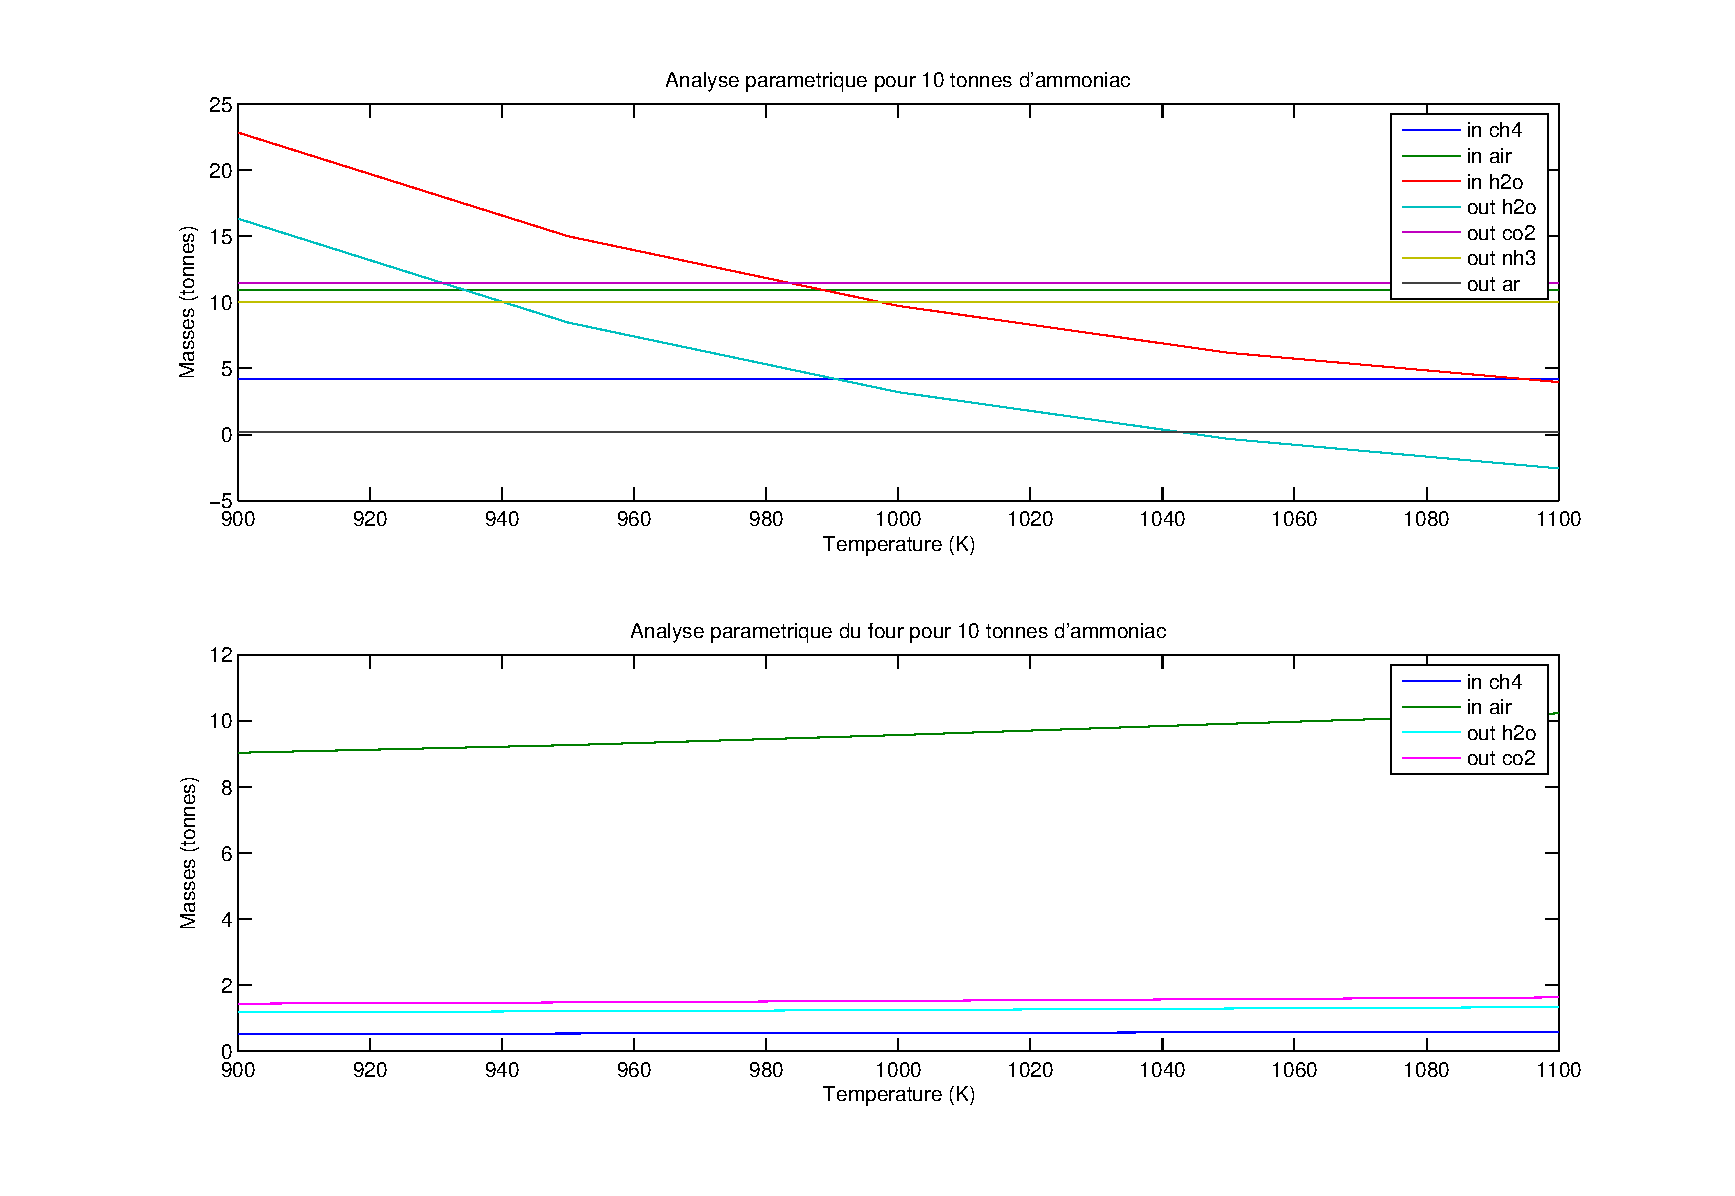
\includegraphics[scale=0.5]{../tache1/img/analyseParam.eps}
	\end{center}
	\caption{Analyse paramétrique pour $10$ tonnes de \ce{NH3}
		le graphe supérieur représente les flux de l'ensemble du 
		procédé, depuis le reformeur primaire jusqu'au réacteur de synthèse.}
	\label{fig:analyseParam}
\end{figure}




\section{Flow-sheet}
\label{sec:flowsheet}

La figure \ref{fig:flowsheet} présente un flow-sheet simplifié du processus 
de production d'ammoniac que nous étudions.

\begin{figure}
	\begin{center}
		\begin{tikzpicture}
[node distance = 7em]

\tikzstyle{output} = [diamond, draw, fill=blue!20, 
    text width=3em, text badly centered, node distance=3cm, inner sep=0pt]
\tikzstyle{block} = [rectangle, draw, fill=blue!20, 
    text width=15em, text centered, rounded corners, minimum height=4em]
\tikzstyle{line} = [draw, -latex']
\tikzstyle{input} = [draw, ellipse,fill=red!20, node distance=3cm,
    minimum height=2em]
    
\node [block] (primaire) {Reformage primaire (T)\\
	\ce{CH4 + H2O <=> CO + 3H2} \\
	\ce{CO + H2O <=> CO2 + H2}};
\node [input, left = 2em of primaire] (H2O) {\ce{H2O}};
\node [block, right = 2em of primaire] (four) {Four: Combustion \ce{CH4} ($\eta = 75\%$) 
($\simeq 1300K$)\\
	\ce{CH4 + 2O2 -> CO2 + 2H2O}};
\node [input, above = 3em of four] (O2) {\ce{O2}};
\node [input, above = 3em of primaire] (CH4) {\ce{CH4}};
\node [block, below of=primaire] (secondaire) {Reformage secondaire ($\simeq 1200K$)\\
	\ce{2CH4 + O2 -> 2CO + 4H2}};
\node [input, right = 1em of secondaire] (air) {Air ($21\% \ce{O2} 78\% \ce{N2} 
	1\% \ce{Ar}$)};
\node [block, below of=secondaire] (wgs) {Water-Gas-Shift ($\simeq 500-700K$)
	\ce{CO + H2O -> CO2 + H2}};
\node [block, below of=wgs] (abso) {Absorbtion du \ce{CO2} et compression};	
\node [output, right = 2em of abso] (CO22) {\ce{CO2}};	
\node [output, left = 2em of abso] (H2O2) {\ce{H2O}};
\node [block, below of=abso] (synthese) {Synthèse \ce{NH3} et séparation de l'argon \\
(Sortie réacteur: 270bar, 750K) \\
	\ce{3H2 + N2 <=> 2NH3}};
\node [output, below of=synthese] (NH3) {\ce{NH3}};
\node [output, right = 2em of synthese] (argon) {\ce{Ar}};


\path [line] (primaire) -- node[anchor = east] {\ce{H2} \ce{CH4} \ce{CO2} \ce{CO} \ce{H2O}}
	(secondaire);
\path [line] (four) -- node[anchor = south] {\textbf{E}}(primaire);
\path [line,dashed] (CH4) -- (four);
\path [line,dashed] (CH4) -- (primaire);
\path [line,dashed] (O2) -- (four);
\path [line] (secondaire) -- node[anchor = east] {\ce{H2} \ce{N2} \ce{CO2} \ce{CO} \ce{Ar} 
	\ce{H2O}}(wgs);
\path [line] (wgs) -- node[anchor = east] {\ce{H2} \ce{H2O} \ce{CO2} \ce{N2} \ce{Ar}}(abso);
\path [line] (abso) -- node[anchor = east] {\ce{H2} \ce{N2} \ce{Ar}}(synthese);
\path [line,dashed] (synthese) -- (NH3);
\path [line,dashed] (synthese) -- (argon);
\path [line,dashed] (air) -- (secondaire);
\path [line,dashed] (H2O) -- (primaire);
\path [line,dashed] (abso) -- (CO22);
\path [line,dashed] (abso) -- (H2O2);

\end{tikzpicture}


	\end{center}
	\caption{Flow-sheet simplifié.}
	\label{fig:flowsheet}
\end{figure}

